% Options for packages loaded elsewhere
\PassOptionsToPackage{unicode}{hyperref}
\PassOptionsToPackage{hyphens}{url}
%
\documentclass[
]{article}
\usepackage{amsmath,amssymb}
\usepackage{lmodern}
\usepackage{iftex}
\ifPDFTeX
  \usepackage[T1]{fontenc}
  \usepackage[utf8]{inputenc}
  \usepackage{textcomp} % provide euro and other symbols
\else % if luatex or xetex
  \usepackage{unicode-math}
  \defaultfontfeatures{Scale=MatchLowercase}
  \defaultfontfeatures[\rmfamily]{Ligatures=TeX,Scale=1}
\fi
% Use upquote if available, for straight quotes in verbatim environments
\IfFileExists{upquote.sty}{\usepackage{upquote}}{}
\IfFileExists{microtype.sty}{% use microtype if available
  \usepackage[]{microtype}
  \UseMicrotypeSet[protrusion]{basicmath} % disable protrusion for tt fonts
}{}
\makeatletter
\@ifundefined{KOMAClassName}{% if non-KOMA class
  \IfFileExists{parskip.sty}{%
    \usepackage{parskip}
  }{% else
    \setlength{\parindent}{0pt}
    \setlength{\parskip}{6pt plus 2pt minus 1pt}}
}{% if KOMA class
  \KOMAoptions{parskip=half}}
\makeatother
\usepackage{xcolor}
\usepackage[margin=1in]{geometry}
\usepackage{color}
\usepackage{fancyvrb}
\newcommand{\VerbBar}{|}
\newcommand{\VERB}{\Verb[commandchars=\\\{\}]}
\DefineVerbatimEnvironment{Highlighting}{Verbatim}{commandchars=\\\{\}}
% Add ',fontsize=\small' for more characters per line
\usepackage{framed}
\definecolor{shadecolor}{RGB}{248,248,248}
\newenvironment{Shaded}{\begin{snugshade}}{\end{snugshade}}
\newcommand{\AlertTok}[1]{\textcolor[rgb]{0.94,0.16,0.16}{#1}}
\newcommand{\AnnotationTok}[1]{\textcolor[rgb]{0.56,0.35,0.01}{\textbf{\textit{#1}}}}
\newcommand{\AttributeTok}[1]{\textcolor[rgb]{0.77,0.63,0.00}{#1}}
\newcommand{\BaseNTok}[1]{\textcolor[rgb]{0.00,0.00,0.81}{#1}}
\newcommand{\BuiltInTok}[1]{#1}
\newcommand{\CharTok}[1]{\textcolor[rgb]{0.31,0.60,0.02}{#1}}
\newcommand{\CommentTok}[1]{\textcolor[rgb]{0.56,0.35,0.01}{\textit{#1}}}
\newcommand{\CommentVarTok}[1]{\textcolor[rgb]{0.56,0.35,0.01}{\textbf{\textit{#1}}}}
\newcommand{\ConstantTok}[1]{\textcolor[rgb]{0.00,0.00,0.00}{#1}}
\newcommand{\ControlFlowTok}[1]{\textcolor[rgb]{0.13,0.29,0.53}{\textbf{#1}}}
\newcommand{\DataTypeTok}[1]{\textcolor[rgb]{0.13,0.29,0.53}{#1}}
\newcommand{\DecValTok}[1]{\textcolor[rgb]{0.00,0.00,0.81}{#1}}
\newcommand{\DocumentationTok}[1]{\textcolor[rgb]{0.56,0.35,0.01}{\textbf{\textit{#1}}}}
\newcommand{\ErrorTok}[1]{\textcolor[rgb]{0.64,0.00,0.00}{\textbf{#1}}}
\newcommand{\ExtensionTok}[1]{#1}
\newcommand{\FloatTok}[1]{\textcolor[rgb]{0.00,0.00,0.81}{#1}}
\newcommand{\FunctionTok}[1]{\textcolor[rgb]{0.00,0.00,0.00}{#1}}
\newcommand{\ImportTok}[1]{#1}
\newcommand{\InformationTok}[1]{\textcolor[rgb]{0.56,0.35,0.01}{\textbf{\textit{#1}}}}
\newcommand{\KeywordTok}[1]{\textcolor[rgb]{0.13,0.29,0.53}{\textbf{#1}}}
\newcommand{\NormalTok}[1]{#1}
\newcommand{\OperatorTok}[1]{\textcolor[rgb]{0.81,0.36,0.00}{\textbf{#1}}}
\newcommand{\OtherTok}[1]{\textcolor[rgb]{0.56,0.35,0.01}{#1}}
\newcommand{\PreprocessorTok}[1]{\textcolor[rgb]{0.56,0.35,0.01}{\textit{#1}}}
\newcommand{\RegionMarkerTok}[1]{#1}
\newcommand{\SpecialCharTok}[1]{\textcolor[rgb]{0.00,0.00,0.00}{#1}}
\newcommand{\SpecialStringTok}[1]{\textcolor[rgb]{0.31,0.60,0.02}{#1}}
\newcommand{\StringTok}[1]{\textcolor[rgb]{0.31,0.60,0.02}{#1}}
\newcommand{\VariableTok}[1]{\textcolor[rgb]{0.00,0.00,0.00}{#1}}
\newcommand{\VerbatimStringTok}[1]{\textcolor[rgb]{0.31,0.60,0.02}{#1}}
\newcommand{\WarningTok}[1]{\textcolor[rgb]{0.56,0.35,0.01}{\textbf{\textit{#1}}}}
\usepackage{graphicx}
\makeatletter
\def\maxwidth{\ifdim\Gin@nat@width>\linewidth\linewidth\else\Gin@nat@width\fi}
\def\maxheight{\ifdim\Gin@nat@height>\textheight\textheight\else\Gin@nat@height\fi}
\makeatother
% Scale images if necessary, so that they will not overflow the page
% margins by default, and it is still possible to overwrite the defaults
% using explicit options in \includegraphics[width, height, ...]{}
\setkeys{Gin}{width=\maxwidth,height=\maxheight,keepaspectratio}
% Set default figure placement to htbp
\makeatletter
\def\fps@figure{htbp}
\makeatother
\setlength{\emergencystretch}{3em} % prevent overfull lines
\providecommand{\tightlist}{%
  \setlength{\itemsep}{0pt}\setlength{\parskip}{0pt}}
\setcounter{secnumdepth}{-\maxdimen} % remove section numbering
\ifLuaTeX
  \usepackage{selnolig}  % disable illegal ligatures
\fi
\IfFileExists{bookmark.sty}{\usepackage{bookmark}}{\usepackage{hyperref}}
\IfFileExists{xurl.sty}{\usepackage{xurl}}{} % add URL line breaks if available
\urlstyle{same} % disable monospaced font for URLs
\hypersetup{
  pdftitle={SEM Beispiel 1},
  hidelinks,
  pdfcreator={LaTeX via pandoc}}

\title{SEM Beispiel 1}
\author{}
\date{\vspace{-2.5em}2023-06-14}

\begin{document}
\maketitle

\hypertarget{motivation}{%
\subsection{Motivation}\label{motivation}}

Angenommen, du bist ein Forscher, der die Auswirkungen der Herkunft der
Schüler auf die schulischen Leistungen untersucht. Du bekommst ein
Datensatz von Schülern mit jeweils 9 beobachteten Variablen hochgeladen:
Motivation, Harmonie, Stabilität, negative elterliche Psychologie, SES,
verbaler IQ, Lesen, Arithmetik und Rechtschreibung. Der Studienleiter
geht von drei latenten Konstrukten aus: Anpassung, Risiko und Leistung,
die mit der folgenden Codebuch-Zuordnung gemessen werden:

Anpassung

\begin{itemize}
\tightlist
\item
  \texttt{motiv} Motivation
\item
  \texttt{harm} Harmony
\item
  \texttt{stabi} Stability
\end{itemize}

Risiko

\begin{itemize}
\tightlist
\item
  \texttt{ppsych} (Negative) Parental Psychology
\item
  \texttt{ses} SES
\item
  \texttt{verbal} Verbal IQ
\end{itemize}

Leistung

\begin{itemize}
\tightlist
\item
  \texttt{read} Reading
\item
  \texttt{arith} Arithmetic
\item
  \texttt{spell} Spelling
\end{itemize}

Anschauen des Datensatzes

\begin{Shaded}
\begin{Highlighting}[]
\FunctionTok{set.seed}\NormalTok{(}\DecValTok{42}\NormalTok{)    }\CommentTok{\# Niemals vergessen!}
\FunctionTok{summary}\NormalTok{(dat)}
\end{Highlighting}
\end{Shaded}

\begin{verbatim}
##      motiv               harm               stabi              ppsych        
##  Min.   :-33.9712   Min.   :-32.98229   Min.   :-25.9214   Min.   :-31.0939  
##  1st Qu.: -7.1480   1st Qu.: -6.05006   1st Qu.: -6.9361   1st Qu.: -6.5397  
##  Median :  0.3155   Median :  0.00679   Median :  0.3016   Median : -0.5439  
##  Mean   :  0.0000   Mean   :  0.00000   Mean   :  0.0000   Mean   :  0.0000  
##  3rd Qu.:  6.7085   3rd Qu.:  6.62110   3rd Qu.:  7.4554   3rd Qu.:  6.7307  
##  Max.   : 26.4690   Max.   : 31.16372   Max.   : 29.6349   Max.   : 33.2828  
##       ses               verbal               read             arith         
##  Min.   :-32.1370   Min.   :-37.60733   Min.   :-32.839   Min.   :-26.7009  
##  1st Qu.: -6.3284   1st Qu.: -6.86543   1st Qu.: -6.843   1st Qu.: -6.4011  
##  Median : -0.3117   Median :  0.04975   Median : -0.043   Median :  0.1266  
##  Mean   :  0.0000   Mean   :  0.00000   Mean   :  0.000   Mean   :  0.0000  
##  3rd Qu.:  6.3039   3rd Qu.:  6.23002   3rd Qu.:  6.657   3rd Qu.:  6.5697  
##  Max.   : 29.0963   Max.   : 27.65674   Max.   : 27.606   Max.   : 33.0483  
##      spell           
##  Min.   :-31.360980  
##  1st Qu.: -6.318838  
##  Median : -0.009114  
##  Mean   :  0.000000  
##  3rd Qu.:  6.340824  
##  Max.   : 26.932760
\end{verbatim}

Die wichtigste Komponente eines Strukturgleichungsmodells ist die
Kovarianz bzw. die statistische Beziehung zwischen den Größen.

Die wahre Kovarianz der Population, bezeichnet als bezeichnet, wird als
Varianz-Kovarianz-Matrix bezeichnet. Da wir diese nicht wissen, müssen
wir sie mit unserer Stichprobe schätzen die sogenannte
Varianz-Kovarianz-Matrix der Stichprobe. Die Funktion \texttt{cov} gibt
an, dass wir die Kovarianzmatrix aus den Daten erhalten wollen.

\begin{Shaded}
\begin{Highlighting}[]
\FunctionTok{cov}\NormalTok{(dat)}
\end{Highlighting}
\end{Shaded}

\begin{verbatim}
##        motiv harm stabi ppsych ses verbal read arith spell
## motiv    100   77    59    -25  25     32   53    60    59
## harm      77  100    58    -25  26     25   42    44    45
## stabi     59   58   100    -16  18     27   36    38    38
## ppsych   -25  -25   -16    100 -42    -40  -39   -24   -31
## ses       25   26    18    -42 100     40   43    37    33
## verbal    32   25    27    -40  40    100   56    49    48
## read      53   42    36    -39  43     56  100    73    87
## arith     60   44    38    -24  37     49   73   100    72
## spell     59   45    38    -31  33     48   87    72   100
\end{verbatim}

\hypertarget{interpretation}{%
\paragraph{Interpretation}\label{interpretation}}

Die Diagonalen bilden die Varianzen der Items und die Off-Diagonalen die
Kovarianzen. Beachte, dass die Varianz aller Variablen in unserer Studie
zufällig 100 beträgt (entlang der Diagonalen). Betrachtet man die
Beziehungen zwischen den Variablen (die Elemente auf den
Außendiagonalen), so ist zu beachten, dass eine positive Kovarianz
bedeutet, dass ein Element zunimmt, wenn das andere zunimmt, eine
negative Kovarianz bedeutet, dass ein Element zunimmt, wenn das andere
abnimmt. Die Kovarianz von \texttt{motiv} und \texttt{ppsych} beträgt
\texttt{-25}, was bedeutet, dass die Motivation der Schüler mit
zunehmender negativer elterlicher Psychologie abnimmt.

\(\rightarrow\) Weiter in den Slides.

\begin{center}\rule{0.5\linewidth}{0.5pt}\end{center}

\hypertarget{simple-regression}{%
\subsection{Simple regression}\label{simple-regression}}

Weiter mit dem Beispiel aus den Slides.

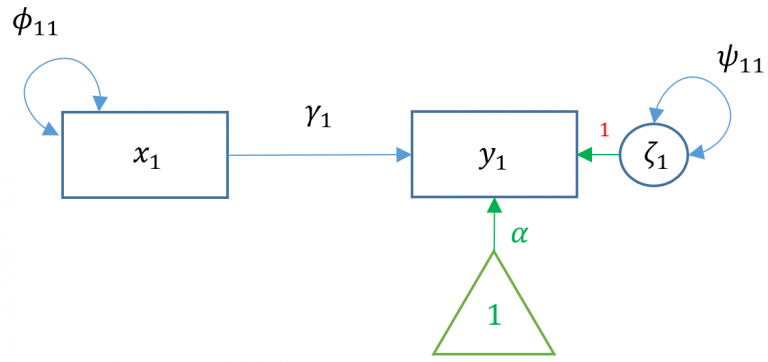
\includegraphics[width=0.6\textwidth,height=\textheight]{lisrel_bsp.png}

Wir bauen ein einfaches Lineares Modell

\begin{Shaded}
\begin{Highlighting}[]
\NormalTok{m1a }\OtherTok{\textless{}{-}} \FunctionTok{lm}\NormalTok{(read }\SpecialCharTok{\textasciitilde{}}\NormalTok{ motiv, }\AttributeTok{data=}\NormalTok{dat)}
\FunctionTok{summary}\NormalTok{(m1a)}
\end{Highlighting}
\end{Shaded}

\begin{verbatim}
## 
## Call:
## lm(formula = read ~ motiv, data = dat)
## 
## Residuals:
##      Min       1Q   Median       3Q      Max 
## -26.0995  -6.1109   0.2342   5.2237  24.0183 
## 
## Coefficients:
##               Estimate Std. Error t value Pr(>|t|)    
## (Intercept) -1.232e-07  3.796e-01    0.00        1    
## motiv        5.300e-01  3.800e-02   13.95   <2e-16 ***
## ---
## Signif. codes:  0 '***' 0.001 '**' 0.01 '*' 0.05 '.' 0.1 ' ' 1
## 
## Residual standard error: 8.488 on 498 degrees of freedom
## Multiple R-squared:  0.2809, Adjusted R-squared:  0.2795 
## F-statistic: 194.5 on 1 and 498 DF,  p-value: < 2.2e-16
\end{verbatim}

Wir können das selbe Modell auch mit dem \texttt{lavaan} Package bauen.
Dieses Package ist extra dafür gebaut worden um SEMs zu bauen und zu
nutzen.

\begin{Shaded}
\begin{Highlighting}[]
\CommentTok{\# Generelle Schreibweise:}
\DocumentationTok{\#\# Modellgleichung}
\NormalTok{mgl }\OtherTok{\textless{}{-}} \StringTok{\textquotesingle{}\# regressions}
\StringTok{       y \textasciitilde{} 1 + Variablen}
\StringTok{       \# variance (optional)}
\StringTok{       Variable(n) \textasciitilde{}\textasciitilde{} Variable(n)\textquotesingle{}}
\DocumentationTok{\#\# Modell Fitten}
\NormalTok{model }\OtherTok{\textless{}{-}} \FunctionTok{sem}\NormalTok{(mgl, }\AttributeTok{data=}\NormalTok{datensatz)}
\end{Highlighting}
\end{Shaded}

Die Syntax ist \texttt{lm()} insofern sehr ähnlich, als
\texttt{read\ \textasciitilde{}\ motiv} den Prädiktor motiv auf das
Ergebnis read angibt. Der Intercept ist jedoch standardmäßig nicht in
der Ausgabe enthalten, sondern wird impliziert. Wenn wir einen Intercept
hinzufügen wollen, müssen wir
\texttt{read\ \textasciitilde{}\ 1\ +\ motiv} einschließen. Optional
können Sie die Varianz von motiv mit
\texttt{motiv\ \textasciitilde{}\textasciitilde{}\ motiv} abfragen. Wenn
diese Syntax nicht angegeben wird, wird der Parameter zwar geschätzt,
aber nur implizit angegeben.

\begin{Shaded}
\begin{Highlighting}[]
\FunctionTok{library}\NormalTok{(lavaan)}
\end{Highlighting}
\end{Shaded}

\begin{verbatim}
## This is lavaan 0.6-15
## lavaan is FREE software! Please report any bugs.
\end{verbatim}

\begin{Shaded}
\begin{Highlighting}[]
\NormalTok{fit1b }\OtherTok{\textless{}{-}} \FunctionTok{sem}\NormalTok{(}\FunctionTok{c}\NormalTok{(}\StringTok{\textquotesingle{}\# Regressions part}
\StringTok{                read \textasciitilde{} 1 + motiv}
\StringTok{                \# Varianz (optional)}
\StringTok{                motiv \textasciitilde{}\textasciitilde{} motiv\textquotesingle{}}\NormalTok{), }
             \AttributeTok{data=}\NormalTok{dat)}
\FunctionTok{summary}\NormalTok{(fit1b)}
\end{Highlighting}
\end{Shaded}

\begin{verbatim}
## lavaan 0.6.15 ended normally after 8 iterations
## 
##   Estimator                                         ML
##   Optimization method                           NLMINB
##   Number of model parameters                         5
## 
##   Number of observations                           500
## 
## Model Test User Model:
##                                                       
##   Test statistic                                 0.000
##   Degrees of freedom                                 0
## 
## Parameter Estimates:
## 
##   Standard errors                             Standard
##   Information                                 Expected
##   Information saturated (h1) model          Structured
## 
## Regressions:
##                    Estimate  Std.Err  z-value  P(>|z|)
##   read ~                                              
##     motiv             0.530    0.038   13.975    0.000
## 
## Intercepts:
##                    Estimate  Std.Err  z-value  P(>|z|)
##    .read             -0.000    0.379   -0.000    1.000
##     motiv             0.000    0.447    0.000    1.000
## 
## Variances:
##                    Estimate  Std.Err  z-value  P(>|z|)
##     motiv            99.800    6.312   15.811    0.000
##    .read             71.766    4.539   15.811    0.000
\end{verbatim}

Der Achsenabschnitt von \texttt{.read\ (-0,000)} und der
Regressionskoeffizient von
\texttt{read\ \textasciitilde{}\ motiv\ (0,530)} entsprechen mit kleinen
Rundungsfehlern der Ausgabe von \texttt{lm()}. Beachten Sie, dass das
\texttt{.} vor dem Parameter eine endogene Variable unter
Achsenabschnitte und eine Restvarianz unter Varianzen oder Kovarianzen
angibt. Der Achsenabschnitt für das \texttt{motiv\ (0,000)} hat kein
\texttt{.} und seine \texttt{Varianz\ (99,800)} auch nicht, was
bedeutet, dass es sich um einen exogenen Mittelwert und eine exogene
Varianz handelt. Der exogene Mittelwert und die exogene Varianz sollten
eng mit dem univariaten Mittelwert (0) und der Varianz (100)
übereinstimmen, wie unten gezeigt:

\begin{Shaded}
\begin{Highlighting}[]
\FunctionTok{mean}\NormalTok{(dat}\SpecialCharTok{$}\NormalTok{motiv)}
\end{Highlighting}
\end{Shaded}

\begin{verbatim}
## [1] 2.4e-07
\end{verbatim}

\begin{Shaded}
\begin{Highlighting}[]
\FunctionTok{var}\NormalTok{(dat}\SpecialCharTok{$}\NormalTok{motiv)}
\end{Highlighting}
\end{Shaded}

\begin{verbatim}
## [1] 100
\end{verbatim}

\(\rightarrow\) Weiter in den Slides.

\begin{center}\rule{0.5\linewidth}{0.5pt}\end{center}

\hypertarget{multiple-regression}{%
\subsection{Multiple regression}\label{multiple-regression}}

Die einfache Regression ist auf eine einzige exogene Variable
beschränkt. In der Praxis kann ein Forscher daran interessiert sein, wie
eine Gruppe von exogenen Variablen ein Ergebnis vorhersagt. Angenommen,
wir haben immer noch ein endogenes Ergebnis, aber zwei oder mehr exogene
Prädiktoren; dies wird als multiple Regression bezeichnet (nicht zu
verwechseln mit multivariater Regression). Die Matrixform ermöglicht es
uns, die Gleichung für alle Beobachtungen prägnant darzustellen \[
  y_1 = \alpha_1 + \mathbf{x \gamma} + \zeta_1
\]

Angenommen, wir haben zwei exogene Variablen die eine einzige endogene
Variable vorhersagen. Das Pfaddiagramm für diese multiple Regression
(Modell 2) lautet

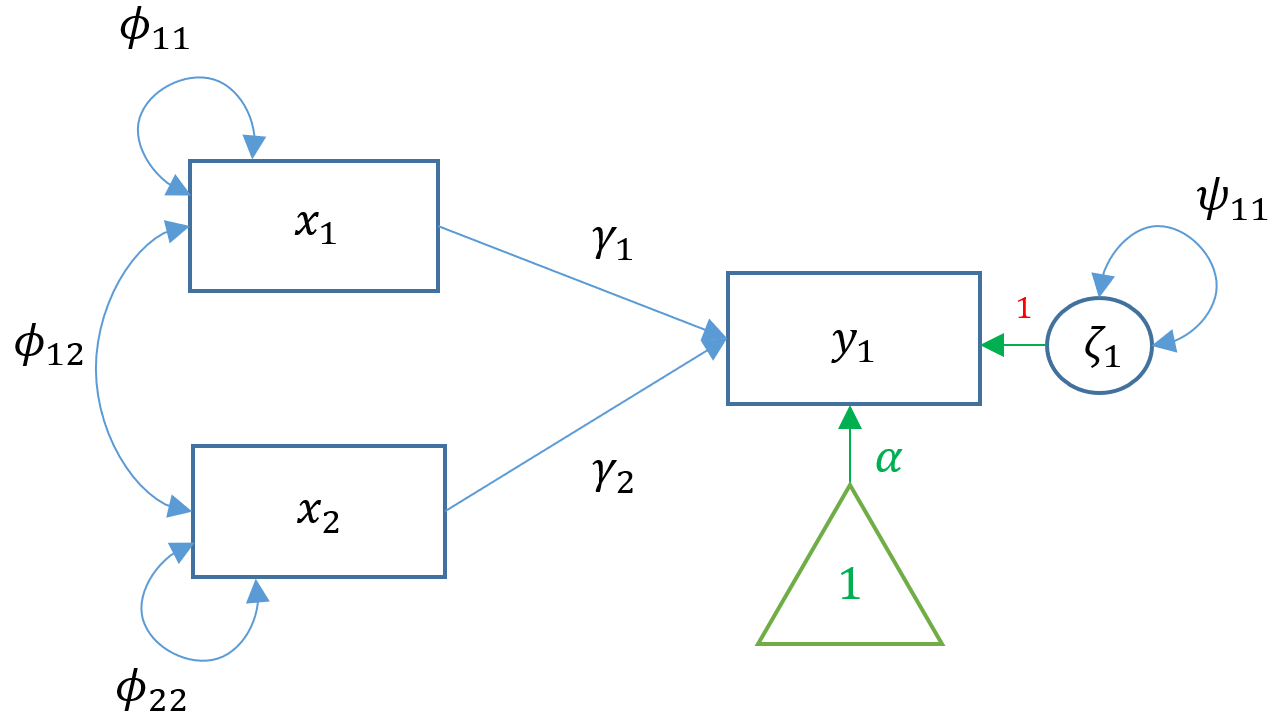
\includegraphics[width=0.6\textwidth,height=\textheight]{m2 (1).png}

Die Spezifikation einer multiplen Regression in Lavaan ist so einfach
wie das Hinzufügen eines weiteren Prädiktors. Angenommen, der Forscher
ist daran interessiert, wie negative elterliche Psychologie
\texttt{ppsych} und \texttt{motiv} motivieren, die Leseergebnisse der
Schüler vorherzusagen.

\begin{Shaded}
\begin{Highlighting}[]
\NormalTok{m2 }\OtherTok{\textless{}{-}} \FunctionTok{sem}\NormalTok{(}\FunctionTok{c}\NormalTok{(}\StringTok{\textquotesingle{}\# regressions}
\StringTok{                read \textasciitilde{} 1 + ppsych + motiv}
\StringTok{                \# covariance}
\StringTok{                ppsych \textasciitilde{}\textasciitilde{} motiv\textquotesingle{}}\NormalTok{), }
             \AttributeTok{data=}\NormalTok{dat)}

\NormalTok{fit2 }\OtherTok{\textless{}{-}} \FunctionTok{sem}\NormalTok{(m2, }\AttributeTok{data=}\NormalTok{dat)}

\FunctionTok{summary}\NormalTok{(fit2)}
\end{Highlighting}
\end{Shaded}

\begin{verbatim}
## lavaan 0.6.15 ended normally after 1 iteration
## 
##   Estimator                                         ML
##   Optimization method                           NLMINB
##   Number of model parameters                         9
## 
##   Number of observations                           500
## 
## Model Test User Model:
##                                                       
##   Test statistic                                 0.000
##   Degrees of freedom                                 0
## 
## Parameter Estimates:
## 
##   Standard errors                             Standard
##   Information                                 Expected
##   Information saturated (h1) model          Structured
## 
## Regressions:
##                    Estimate  Std.Err  z-value  P(>|z|)
##   read ~                                              
##     ppsych           -0.275    0.037   -7.385    0.000
##     motiv             0.461    0.037   12.404    0.000
## 
## Covariances:
##                    Estimate  Std.Err  z-value  P(>|z|)
##   ppsych ~~                                           
##     motiv           -24.950    4.601   -5.423    0.000
## 
## Intercepts:
##                    Estimate  Std.Err  z-value  P(>|z|)
##    .read             -0.000    0.360   -0.000    1.000
##     ppsych           -0.000    0.447   -0.000    1.000
##     motiv             0.000    0.447    0.000    1.000
## 
## Variances:
##                    Estimate  Std.Err  z-value  P(>|z|)
##    .read             64.708    4.092   15.811    0.000
##     ppsych           99.800    6.312   15.811    0.000
##     motiv            99.800    6.312   15.811    0.000
\end{verbatim}

\(\rightarrow\) Weiter in den Slides.

\begin{center}\rule{0.5\linewidth}{0.5pt}\end{center}

Einfache und multiple Regression modellieren jeweils ein Ergebnis
(\(y\)) zu einem Zeitpunkt. Bei der multivariaten oder simultanen
linearen Regression werden mehrere Ergebnisse gleichzeitig modelliert
\(y_1, y_2, \dots, y_p\). Das allgemeine multivariate lineare Modell ist
definiert als
\[\mathbf{y} = \mathbf{\alpha} + \mathbf{\Gamma} \mathbf{x} + \mathbf{\zeta}\]
Um die Matrixformulierung deutlicher zu sehen, betrachten Sie zwei
(d.~h. bivariate) endogene Variablen (\(y_1, y_2\)), die von zwei
exogenen Prädiktoren \(x_1, x_2\) vorhergesagt werden. \$\$

\begin{pmatrix}
    y_{1} \\
    y_{2}
  \end{pmatrix}

=

\begin{pmatrix}
    \alpha_1 \\
    \alpha_2
  \end{pmatrix}

\begin{itemize}
\item
  \begin{pmatrix}
     \gamma_{11} & \gamma_{12}\\
     0 & \gamma_{22}
   \end{pmatrix}
   \begin{pmatrix}
     x_1 \\
     x_2
   \end{pmatrix}

  \begin{itemize}
  \item
    \begin{pmatrix}
      \zeta_{1}\\
      \zeta_{2}
    \end{pmatrix}

    \$\$
  \end{itemize}
\end{itemize}

\(\Gamma\) wird als Strukturparameter bezeichnet und definiert die
Beziehung zwischen exogenen und endogenen Variablen.

\begin{Shaded}
\begin{Highlighting}[]
\NormalTok{m3a }\OtherTok{\textless{}{-}} \StringTok{\textquotesingle{}read \textasciitilde{} 1 + ppsych + motiv}
\StringTok{        arith \textasciitilde{} 1 + motiv\textquotesingle{}}
\NormalTok{fit3a }\OtherTok{\textless{}{-}} \FunctionTok{sem}\NormalTok{(m3a, }\AttributeTok{data=}\NormalTok{dat)}
\FunctionTok{summary}\NormalTok{(fit3a)}
\end{Highlighting}
\end{Shaded}

\begin{verbatim}
## lavaan 0.6.15 ended normally after 17 iterations
## 
##   Estimator                                         ML
##   Optimization method                           NLMINB
##   Number of model parameters                         8
## 
##   Number of observations                           500
## 
## Model Test User Model:
##                                                       
##   Test statistic                                 6.796
##   Degrees of freedom                                 1
##   P-value (Chi-square)                           0.009
## 
## Parameter Estimates:
## 
##   Standard errors                             Standard
##   Information                                 Expected
##   Information saturated (h1) model          Structured
## 
## Regressions:
##                    Estimate  Std.Err  z-value  P(>|z|)
##   read ~                                              
##     ppsych           -0.216    0.030   -7.289    0.000
##     motiv             0.476    0.037   12.918    0.000
##   arith ~                                             
##     motiv             0.600    0.036   16.771    0.000
## 
## Covariances:
##                    Estimate  Std.Err  z-value  P(>|z|)
##  .read ~~                                             
##    .arith            39.179    3.373   11.615    0.000
## 
## Intercepts:
##                    Estimate  Std.Err  z-value  P(>|z|)
##    .read             -0.000    0.361   -0.000    1.000
##    .arith            -0.000    0.357   -0.000    1.000
## 
## Variances:
##                    Estimate  Std.Err  z-value  P(>|z|)
##    .read             65.032    4.113   15.811    0.000
##    .arith            63.872    4.040   15.811    0.000
\end{verbatim}

\begin{Shaded}
\begin{Highlighting}[]
\NormalTok{m3b }\OtherTok{\textless{}{-}} \FunctionTok{lm}\NormalTok{(read }\SpecialCharTok{\textasciitilde{}}\NormalTok{ ppsych }\SpecialCharTok{+}\NormalTok{ motiv, }\AttributeTok{data=}\NormalTok{dat)}
\NormalTok{(fit3b }\OtherTok{\textless{}{-}} \FunctionTok{summary}\NormalTok{(m3b))}
\end{Highlighting}
\end{Shaded}

\begin{verbatim}
## 
## Call:
## lm(formula = read ~ ppsych + motiv, data = dat)
## 
## Residuals:
##      Min       1Q   Median       3Q      Max 
## -21.7734  -5.5633   0.1389   5.3662  25.8209 
## 
## Coefficients:
##               Estimate Std. Error t value Pr(>|t|)    
## (Intercept) -1.336e-07  3.608e-01   0.000        1    
## ppsych      -2.747e-01  3.730e-02  -7.363 7.51e-13 ***
## motiv        4.613e-01  3.730e-02  12.367  < 2e-16 ***
## ---
## Signif. codes:  0 '***' 0.001 '**' 0.01 '*' 0.05 '.' 0.1 ' ' 1
## 
## Residual standard error: 8.068 on 497 degrees of freedom
## Multiple R-squared:  0.3516, Adjusted R-squared:  0.349 
## F-statistic: 134.8 on 2 and 497 DF,  p-value: < 2.2e-16
\end{verbatim}

Führen wir nun das Modell von arith auf motiv in lm() aus

\begin{Shaded}
\begin{Highlighting}[]
\NormalTok{m3c }\OtherTok{\textless{}{-}} \FunctionTok{lm}\NormalTok{(arith }\SpecialCharTok{\textasciitilde{}}\NormalTok{ motiv, }\AttributeTok{data=}\NormalTok{dat)}
\NormalTok{(fit3c }\OtherTok{\textless{}{-}} \FunctionTok{summary}\NormalTok{(m3c))}
\end{Highlighting}
\end{Shaded}

\begin{verbatim}
## 
## Call:
## lm(formula = arith ~ motiv, data = dat)
## 
## Residuals:
##     Min      1Q  Median      3Q     Max 
## -23.633  -5.341  -0.214   5.106  21.271 
## 
## Coefficients:
##               Estimate Std. Error t value Pr(>|t|)    
## (Intercept) -5.400e-08  3.581e-01    0.00        1    
## motiv        6.000e-01  3.585e-02   16.74   <2e-16 ***
## ---
## Signif. codes:  0 '***' 0.001 '**' 0.01 '*' 0.05 '.' 0.1 ' ' 1
## 
## Residual standard error: 8.008 on 498 degrees of freedom
## Multiple R-squared:   0.36,  Adjusted R-squared:  0.3587 
## F-statistic: 280.1 on 1 and 498 DF,  p-value: < 2.2e-16
\end{verbatim}

Wir sehen, dass der Koeffizient
\texttt{read\ \textasciitilde{}\textasciitilde{}\ ppsych} in Lavaan
\texttt{-0,216} beträgt, in Lavaan aber \texttt{-0,2747}. Könnte dies
ein Rundungsfehler sein? Betrachtet man außerdem die Standardfehler der
Residuen, so stellt man fest, dass die Restvarianz von \texttt{arith}
\texttt{8.008\^{}2=64.12} was sich von der \texttt{lavaan}-Schätzung von
\texttt{63.872} unterscheidet. Was könnte die Ursache für diesen
Unterschied sein, wenn man weiß, was man aus dem vorherigen Abschnitt
weiß?

\(\rightarrow\) Weiter in den Slides.

\begin{center}\rule{0.5\linewidth}{0.5pt}\end{center}

\hypertarget{multivariate-regression-zur-entfernung-von-standardkovarianzen}{%
\subsection{Multivariate Regression zur Entfernung von
Standardkovarianzen}\label{multivariate-regression-zur-entfernung-von-standardkovarianzen}}

Eine Antwort auf die obrige Frage ist dass \texttt{lm()} den
Klein-Quadrate Schätzer benutzt, während \texttt{laavan}auf der
Maximum-likelihood Methode basiert, daher der Unterschied in den
Schätzungen der Restvarianz. Unabhängig davon, welcher der beiden
Schätzer verwendet wird, sollten die Regressionskoeffizienten jedoch
unverzerrt sein, so dass der Unterschied in den Koeffizienten auf etwas
anderes zurückzuführen sein muss. Die Antwort liegt in der impliziten
Tatsache, dass lavaan standardmäßig die Residualvarianzen der endogenen
Variablen \texttt{.read\ \textasciitilde{}\textasciitilde{}\ .arith}
kovariiert. Entfernt man die Standard-Residualkovarianzen, sieht man im
Pfaddiagramm.

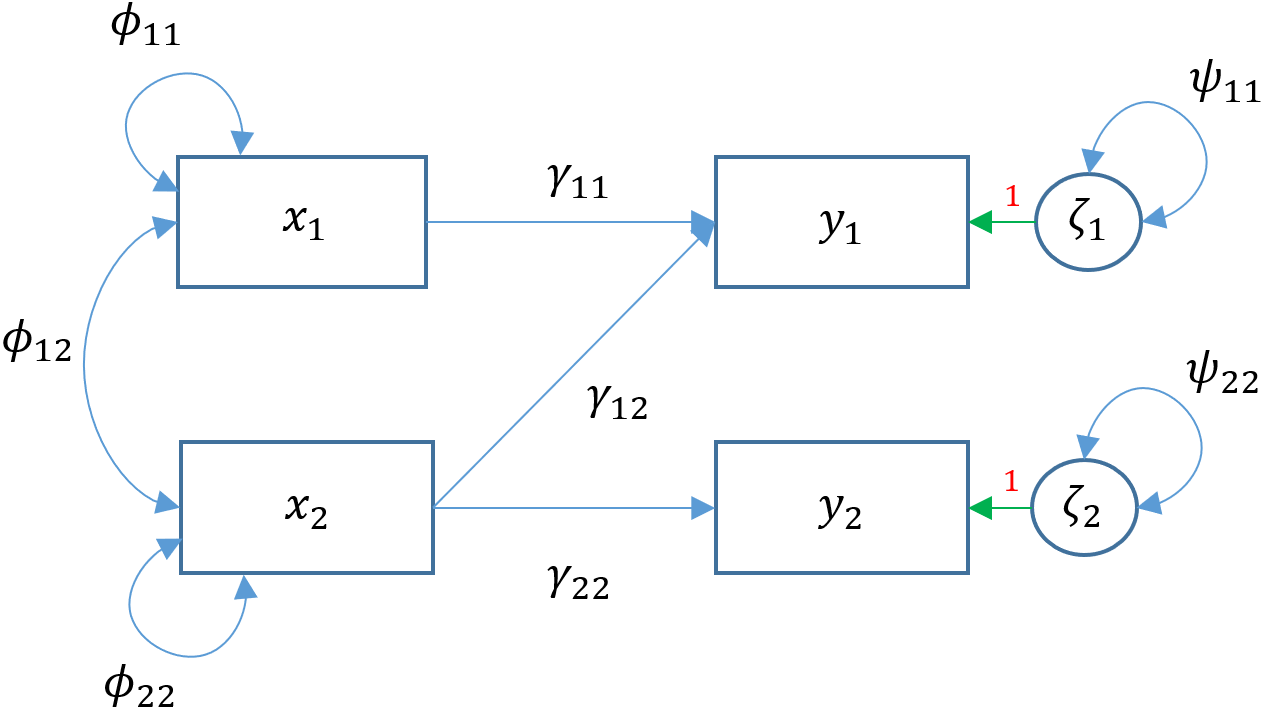
\includegraphics[width=0.6\textwidth,height=\textheight]{m3d.png}

Removing the covariance of \texttt{read} and \texttt{arith} is the same
as fixing its covariance to zero through the following syntax
\texttt{read\ \textasciitilde{}\textasciitilde{}\ 0*arith}.

\begin{Shaded}
\begin{Highlighting}[]
\NormalTok{m3d }\OtherTok{\textless{}{-}} \StringTok{\textquotesingle{}\# regressions}
\StringTok{        read \textasciitilde{} 1 + ppsych + motiv}
\StringTok{        arith \textasciitilde{} 1 + motiv}
\StringTok{        \# covariance}
\StringTok{        read \textasciitilde{}\textasciitilde{} 0*arith }
\StringTok{        \textquotesingle{}}

\NormalTok{fit3d }\OtherTok{\textless{}{-}} \FunctionTok{sem}\NormalTok{(m3d, }\AttributeTok{data=}\NormalTok{dat)}

\FunctionTok{summary}\NormalTok{(fit3d)}
\end{Highlighting}
\end{Shaded}

\begin{verbatim}
## lavaan 0.6.15 ended normally after 2 iterations
## 
##   Estimator                                         ML
##   Optimization method                           NLMINB
##   Number of model parameters                         7
## 
##   Number of observations                           500
## 
## Model Test User Model:
##                                                       
##   Test statistic                               234.960
##   Degrees of freedom                                 2
##   P-value (Chi-square)                           0.000
## 
## Parameter Estimates:
## 
##   Standard errors                             Standard
##   Information                                 Expected
##   Information saturated (h1) model          Structured
## 
## Regressions:
##                    Estimate  Std.Err  z-value  P(>|z|)
##   read ~                                              
##     ppsych           -0.275    0.037   -7.385    0.000
##     motiv             0.461    0.037   12.404    0.000
##   arith ~                                             
##     motiv             0.600    0.036   16.771    0.000
## 
## Covariances:
##                    Estimate  Std.Err  z-value  P(>|z|)
##  .read ~~                                             
##    .arith             0.000                           
## 
## Intercepts:
##                    Estimate  Std.Err  z-value  P(>|z|)
##    .read              0.000    0.360    0.000    1.000
##    .arith             0.000    0.357    0.000    1.000
## 
## Variances:
##                    Estimate  Std.Err  z-value  P(>|z|)
##    .read             64.708    4.092   15.811    0.000
##    .arith            63.872    4.040   15.811    0.000
\end{verbatim}

\end{document}
